%\documentclass[aspectratio=43]{beamer}
\documentclass[c]{beamer}
\usetheme{intridea}  %% Themenwahl

\usepackage[ngerman]{babel} 
\usepackage[T1]{fontenc}    % richtige Silbentrennung
\usepackage[utf8]{inputenc} % Umlaute etc.!
\usepackage{eurosym}
\usepackage{tikz}

\usetikzlibrary{arrows,decorations.pathmorphing,backgrounds,fit,positioning,shapes.symbols,chains}

\title{Freifunk Hamburg}
\author{hamburg.freifunk.net}
\date{14. Februar 2013}

%TODO Saetze mit Punkt beenden

\begin{document}
\maketitle

\begin{frame}{Wer sind wir?}
	Arnd Siebke
	\begin{itemize}
		\item Erzieher in einem Hort in Hamburg
	\end{itemize}

	Christopher Schwardt
	\begin{itemize}
		\item Informatikstudent Universität Hamburg
	\end{itemize}

	Andre Müller
	\begin{itemize}
		\item Systemadministrator
	\end{itemize}
\end{frame}

%===================|
% Begin Mchais Part |
%===================|

%2
\begin{frame}{Was ist Freifunk?}
	\begin{itemize}
		\item Freifunk ist eine nicht kommerzielle Initiative zur Förderung freier Netzwerke

		\item Freifunk Hamburg ist eine Projektgruppe des Chaos Computer Club Hamburg

		\item Zusammenarbeit
		%TODO vspace
		\begin{itemize}
			\item Digitale Gesellschaft e.V.
		\end{itemize}
	\end{itemize}
\end{frame}

%2
\begin{frame}{Was ist Freifunk?}
\begin{itemize}
	\item \textbf{frei} wird verstanden als:
	\begin{itemize}
		\item Öffentlich - jedem zugänglich
		\item Nicht kommerziell
		\item Im Besitz der Gemeinschaft
		\item Netzneutral - keine Manipulation der Datenströme
	\end{itemize}
	\item Mit \textbf{Netzwerk} meinen wir:
	\begin{itemize}
		\item Kommunikation zwischen Menschen unter Verwendung digitaler Medien (Computer, Handys, Datennetze)
	\end{itemize}
  \end{itemize}
\end{frame}

%3
\begin{frame}{Ziel des Projekts}
	\begin{itemize}
		\item Verbreitung offener WLAN-Netzwerke
		\item Zugangshürden zum Internet minimieren
		\item Aufklärung und Sensibilisierung zum Thema ``Kommunikations- und Informationsfreiheit''
		\item Menschen dazu befähigen, eigene Netze aufzubauen und zu betreiben
		\item Soziale Strukturen bilden und unterstützen
	\end{itemize}
\end{frame}

%5
\begin{frame}{Warum WLAN?}
	\begin{itemize}
		\item Mit WLAN können Daten mobil mit hoher Bandbreite gesendet und empfangen werden
		\item Die Kosten für WLAN-Hardware sind gering und es entstehen kaum Betriebskosten (Router ab \EUR{15}, Strom \EUR{10} im Jahr)
		\item WLAN kann auch dort eingesetzt werden, wo es keine Kabel gibt oder eine Kabelverbindung zu teuer ist
		%[Parks, Entwicklungsländer, etc...]
	\end{itemize}
\end{frame}

%==================|
% Begin Chriz Part |
%==================|

%10
\begin{frame}{Mesh-Netzwerke}
	\begin{itemize}
		\item to mesh = Englisch: vermaschen
		\item Selbst organisierende Netzwerke
		\item Jeder Router ist automatisch aktiver Teil des Netzwerks
	\end{itemize}
\end{frame}

%11
\begin{frame}{Mesh-Netzwerke}
%	\begin{columns}[c]
%		\begin{column}[c]{0.4\textwidth}
		\begin{center}
			\begin{tikzpicture}
				\definecolor{outerCircleColour}{RGB}{220, 0, 103}
				\definecolor{innerCircleColour}{RGB}{255, 203, 18}
				\tikzstyle{vertex}=[circle, draw, color=outerCircleColour, ultra thick, minimum size=84pt]
				\tikzstyle{place}=[circle, draw, color=innerCircleColour, fill=innerCircleColour, minimum size=6pt, inner sep=0pt]

				\node [vertex] (a) {};
				\node [vertex, xshift=68pt, yshift=24pt] (b) {};
				\node [vertex, xshift=112pt, yshift=-20pt] (c) {};

				\node [place, label=above:$A$] (A) {};
				\node [place, xshift=68pt, yshift=24pt, label=above:$B$] (B) {};
				\node [place, xshift=112pt, yshift=-20pt, label=right:$C$] (C) {};

				\path[-, thick, color=gray]
				(A) edge (B)
				(B) edge (C);
			\end{tikzpicture}
		\end{center}
%		\end{column}
%		\begin{column}[c]{0.5\textwidth}
%			\begin{itemize}
%				\item $A$ kann $B$ erreichen und $B$ erreicht $C$
%				\item Über ``ad-hoc routing''-Protokolle tauschen die Geräte selbstständig Informationen darüber aus, wer wen erreichen kann
%				\item $A$ erreicht automatisch $C$, wenn\\
%				$A$ Kontakt zu $B$ und\\
%				$B$ Kontakt zu $C$ hat
%			\end{itemize}
%		\end{column}
%	\end{columns}
\end{frame}

%12
\begin{frame}{Mesh-Netzwerke}
%	\begin{columns}[c]
%		\begin{column}[c]{.4\textwidth}
		\begin{center}
			\begin{tikzpicture}
\definecolor{outerCircleColour}{RGB}{220, 0, 103}
				\definecolor{innerCircleColour}{RGB}{255, 203, 18}
				\tikzstyle{vertex}=[circle, draw, color=outerCircleColour, ultra thick, minimum size=84pt]
				\tikzstyle{place}=[circle, draw, color=innerCircleColour, fill=innerCircleColour, minimum size=6pt, inner sep=0pt]

				\node [vertex] (a) {};
				\node [vertex, xshift=68pt, yshift=24pt] (b) {};
				\node [vertex, xshift=112pt, yshift=-20pt] (c) {};

				\node [place, label=above:$A$] (A) {};
				\node [place, xshift=68pt, yshift=24pt, label=above:$B$] (B) {};
				\node [place, xshift=112pt, yshift=-20pt, label=right:$C$] (C) {};

				\path[-, thick, color=gray]
				(A) edge (B)
				(B) edge (C)
				(A) edge[dashed] (C);
			\end{tikzpicture}
		\end{center}
%		\end{column}
%		\begin{column}[c]{.5\textwidth}
%			Damit Informationen von einem Ende des Netzes ($A$) zum anderen gelangen können ($C$), muss die dazwischen liegende Knotenpunkte ($B$) den ungehinderten Transfer von Daten erlauben!\\
%			Das machen die Router im Freifunk.
%		\end{column}
%	\end{columns}
\end{frame}

%18
\begin{frame}{Das Netz wächst}
	\begin{tikzpicture}
		\definecolor{outerCircleColour}{RGB}{220, 0, 103}
		\definecolor{innerCircleColour}{RGB}{255, 203, 18}
		\tikzstyle{vertex}=[circle, draw, color=outerCircleColour, ultra thick, minimum size=40pt]
		\tikzstyle{place}=[circle, draw, color=innerCircleColour, fill=innerCircleColour, minimum size=7pt, inner sep=0pt]

		\node [vertex] (a) {};
		\node [vertex, xshift=15pt, yshift=30pt] (b) {};
		\node [vertex, xshift=65pt, yshift=5pt] (c) {};
		\node [vertex, xshift=33pt, yshift=-3pt] (d) {};
		\node [vertex, xshift=85pt, yshift=-25pt] (e) {};
		\node [vertex, xshift=100pt, yshift=2pt] (f) {};
		\node [vertex, xshift=91pt, yshift=32pt] (g) {};
		\node [vertex, xshift=110pt, yshift=-52pt] (h) {};
		\node [vertex, xshift=124pt, yshift=23pt] (i) {};
		\node [vertex, xshift=134pt, yshift=-7pt] (j) {};
		\node [vertex, xshift=164pt, yshift=-14pt] (k) {};
		\node [vertex, xshift=144pt, yshift=-66pt] (l) {};
		\node [vertex, xshift=170pt, yshift=-46pt] (m) {};
		\node [vertex, xshift=201pt, yshift=-59pt] (n) {};

		\node [place] (A) {};
		\node [place, xshift=15pt, yshift=30pt] (B) {};
		\node [place, xshift=65pt, yshift=5pt] (C) {};
		\node [place, xshift=33pt, yshift=-3pt] (D) {};
		\node [place, xshift=85pt, yshift=-25pt] (E) {};
		\node [place, xshift=100pt, yshift=2pt] (F) {};
		\node [place, xshift=91pt, yshift=32pt] (G) {};
		\node [place, xshift=110pt, yshift=-52pt] (H) {};
		\node [place, xshift=124pt, yshift=23pt] (I) {};
		\node [place, xshift=134pt, yshift=-7pt] (J) {};
		\node [place, xshift=164pt, yshift=-14pt] (K) {};
		\node [place, xshift=144pt, yshift=-66pt] (L) {};
		\node [place, xshift=170pt, yshift=-46pt] (M) {};
		\node [place, xshift=201pt, yshift=-59pt] (N) {};

		\path[-, thick, color=gray]
		(A) edge (B)
		(A) edge (D)
		(B) edge (D)
		(C) edge (D)
		(C) edge (E)
		(C) edge (F)
		(C) edge (G)
		(E) edge (F)
		(E) edge (H)
		(F) edge (G)
		(F) edge (I)
		(F) edge (J)
		(G) edge (I)
		(H) edge (L)
		(I) edge (J)
		(J) edge (K)
		(K) edge (M)
		(L) edge (M)
		(M) edge (N);
	\end{tikzpicture}
\end{frame}

%19
\begin{frame}{Netzwerke verbinden sich untereinander}
	\begin{columns}[c]
		\begin{column}[l]{.4\textwidth}
			\scalebox{0.6}[0.6]{
			\begin{tikzpicture}
				\definecolor{outerCircleColour}{RGB}{220, 0, 103}
				\definecolor{innerCircleColour}{RGB}{255, 203, 18}
				\tikzstyle{vertex}=[circle, draw, color=outerCircleColour, ultra thick, minimum size=40pt]
				\tikzstyle{place}=[circle, draw, color=innerCircleColour, fill=innerCircleColour, minimum size=7pt, inner sep=0pt]

				\node [vertex] (a) {};
				\node [vertex, xshift=15pt, yshift=30pt] (b) {};
				\node [vertex, xshift=65pt, yshift=5pt] (c) {};
				\node [vertex, xshift=33pt, yshift=-3pt] (d) {};
				\node [vertex, xshift=85pt, yshift=-25pt] (e) {};
				\node [vertex, xshift=100pt, yshift=2pt] (f) {};
				\node [vertex, xshift=91pt, yshift=32pt] (g) {};
				\node [vertex, xshift=110pt, yshift=-52pt] (h) {};
				\node [vertex, xshift=124pt, yshift=23pt] (i) {};
				\node [vertex, xshift=134pt, yshift=-7pt] (j) {};
				\node [vertex, xshift=164pt, yshift=-14pt] (k) {};
				\node [vertex, xshift=144pt, yshift=-66pt] (l) {};
				\node [vertex, xshift=170pt, yshift=-46pt] (m) {};
				\node [vertex, xshift=201pt, yshift=-59pt] (n) {};

				\node [place] (A) {};
				\node [place, xshift=15pt, yshift=30pt] (B) {};
				\node [place, xshift=65pt, yshift=5pt] (C) {};
				\node [place, xshift=33pt, yshift=-3pt] (D) {};
				\node [place, xshift=85pt, yshift=-25pt] (E) {};
				\node [place, xshift=100pt, yshift=2pt] (F) {};
				\node [place, xshift=91pt, yshift=32pt] (G) {};
				\node [place, xshift=110pt, yshift=-52pt] (H) {};
				\node [place, xshift=124pt, yshift=23pt] (I) {};
				\node [place, xshift=134pt, yshift=-7pt] (J) {};
				\node [place, xshift=164pt, yshift=-14pt] (K) {};
				\node [place, xshift=144pt, yshift=-66pt] (L) {};
				\node [place, xshift=170pt, yshift=-46pt] (M) {};
				\node [place, xshift=201pt, yshift=-59pt] (N) {};

				\path[-, thick, color=gray]
				(A) edge (B)
				(A) edge (D)
				(B) edge (D)
				(C) edge (D)
				(C) edge (E)
				(C) edge (F)
				(C) edge (G)
				(E) edge (F)
				(E) edge (H)
				(F) edge (G)
				(F) edge (I)
				(F) edge (J)
				(G) edge (I)
				(H) edge (L)
				(I) edge (J)
				(J) edge (K)
				(K) edge (M)
				(L) edge (M)
				(M) edge (N);
			\end{tikzpicture}}
		\end{column}
		\begin{column}{0.185\textwidth}
			\begin{uncoverenv}<2->
				\begin{tikzpicture}
					\definecolor{outerCircleColour}{RGB}{220, 0, 103}
					\definecolor{innerCircleColour}{RGB}{255, 203, 18}

					\draw[color=white] (280pt, 85pt) arc (0:0:0pt);
					\draw[color=white] (-180pt, 85pt) arc (0:0:0pt);

					\draw[color=outerCircleColour, thick, xshift=-50pt, yshift=9pt] (-110pt, 0pt) arc (270:450:6pt);
					\draw[color=outerCircleColour, thick, xshift=-50pt, yshift=11pt] (-110pt, 0pt) arc (270:450:4pt);
					\draw[color=outerCircleColour, thick, xshift=-50pt, yshift=13pt] (-110pt, 0pt) arc (270:450:2pt);

					\draw[color=outerCircleColour, thick, xshift=-9pt, yshift=21pt] (-110pt, 0pt) arc (90:270:6pt);
					\draw[color=outerCircleColour, thick, xshift=-9pt, yshift=19pt] (-110pt, 0pt) arc (90:270:4pt);
					\draw[color=outerCircleColour, thick, xshift=-9pt, yshift=17pt] (-110pt, 0pt) arc (90:270:2pt);

					\draw[color=gray, ultra thick, xshift=-50pt, yshift=15] (-103pt, 0pt) edge[dashed] (-74pt, 0pt);
				\end{tikzpicture}
			\end{uncoverenv}
		\end{column}
		\begin{column}[r]{.5\textwidth}
			\reflectbox{
			\scalebox{0.6}[0.6]{
			\begin{tikzpicture}
				\definecolor{outerCircleColour}{RGB}{220, 0, 103}
				\definecolor{innerCircleColour}{RGB}{255, 203, 18}
				\tikzstyle{vertex}=[circle, draw, color=outerCircleColour, ultra thick, minimum size=40pt]
				\tikzstyle{place}=[circle, draw, color=innerCircleColour, fill=innerCircleColour, minimum size=7pt, inner sep=0pt]

				\node [vertex] (a) {};
				\node [vertex, xshift=15pt, yshift=30pt] (b) {};
				\node [vertex, xshift=65pt, yshift=5pt] (c) {};
				\node [vertex, xshift=33pt, yshift=-3pt] (d) {};
				\node [vertex, xshift=85pt, yshift=-25pt] (e) {};
				\node [vertex, xshift=100pt, yshift=2pt] (f) {};
				\node [vertex, xshift=91pt, yshift=32pt] (g) {};
				\node [vertex, xshift=110pt, yshift=-52pt] (h) {};
				\node [vertex, xshift=124pt, yshift=23pt] (i) {};
				\node [vertex, xshift=134pt, yshift=-7pt] (j) {};
				\node [vertex, xshift=164pt, yshift=-14pt] (k) {};
				\node [vertex, xshift=144pt, yshift=-66pt] (l) {};
				\node [vertex, xshift=170pt, yshift=-46pt] (m) {};
				\node [vertex, xshift=201pt, yshift=-59pt] (n) {};

				\node [place] (A) {};
				\node [place, xshift=15pt, yshift=30pt] (B) {};
				\node [place, xshift=65pt, yshift=5pt] (C) {};
				\node [place, xshift=33pt, yshift=-3pt] (D) {};
				\node [place, xshift=85pt, yshift=-25pt] (E) {};
				\node [place, xshift=100pt, yshift=2pt] (F) {};
				\node [place, xshift=91pt, yshift=32pt] (G) {};
				\node [place, xshift=110pt, yshift=-52pt] (H) {};
				\node [place, xshift=124pt, yshift=23pt] (I) {};
				\node [place, xshift=134pt, yshift=-7pt] (J) {};
				\node [place, xshift=164pt, yshift=-14pt] (K) {};
				\node [place, xshift=144pt, yshift=-66pt] (L) {};
				\node [place, xshift=170pt, yshift=-46pt] (M) {};
				\node [place, xshift=201pt, yshift=-59pt] (N) {};

				\path[-, thick, color=gray]
				(A) edge (B)
				(A) edge (D)
				(B) edge (D)
				(C) edge (D)
				(C) edge (E)
				(C) edge (F)
				(C) edge (G)
				(E) edge (F)
				(E) edge (H)
				(F) edge (G)
				(F) edge (I)
				(F) edge (J)
				(G) edge (I)
				(H) edge (L)
				(I) edge (J)
				(J) edge (K)
				(K) edge (M)
				(L) edge (M)
				(M) edge (N);
			\end{tikzpicture}}}
		\end{column}
	\end{columns}
\end{frame}

\begin{frame}{Mit Freifunk ins Internet}
	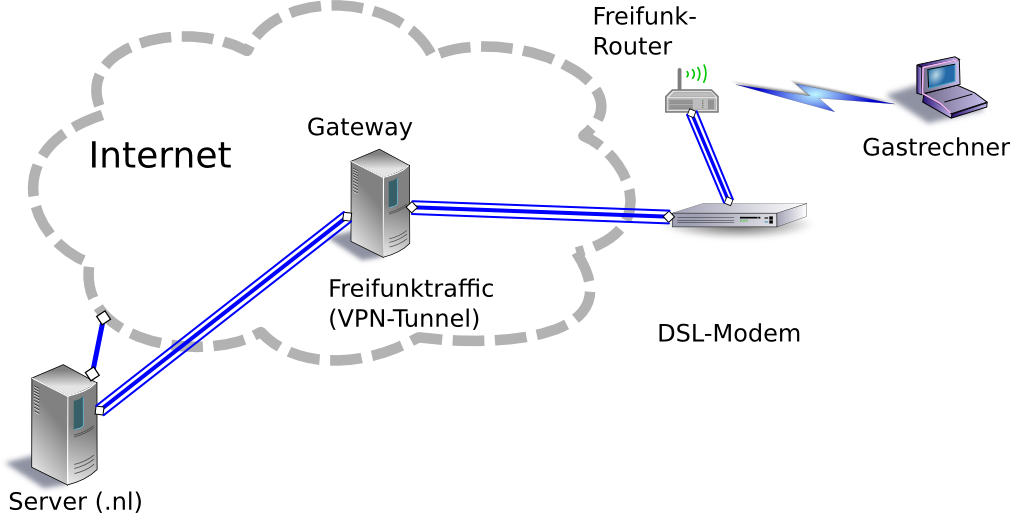
\includegraphics[width=\textwidth]{Freifunk_Knotenanbindung}
\end{frame}

%TODO hier Beispiel von Wilhelmsburg rein
\begin{frame}{Ein Beispiel in Wilhelmsburg}
	\begin{itemize}
		\item IMAGE
	\end{itemize}
\end{frame}

%===================|
% Begin Bashos Part |
%===================|

%13
\begin{frame}{Praktische Umsetzung}
	\begin{itemize}
		\item Sehr häufig verwendet: TL-WR741nd (ca. \EUR{15})
		\item Austausch der vorhandenen Software durch Linux Firmware, die man von unserer Webseite herunterladen kann
		\item Antennen abschraub- und austauschbar
		\item Fertig konfigurierte Router
		\item Vorgefertigte Firmware auch für weitere Router
	\end{itemize}
\end{frame}

%20
\begin{frame}{Die Idee}
	\begin{itemize}
		\item Es entsteht ein eigenes stadtweites Intranet mit lokalen Zugängen ins Internet
		\item Kultureinrichtungen können ein eigenes Programm (Communityradio, Streaming-Media) im Intranet anbieten
		\item Jeder Mensch kann Teil dieses Netzes sein ohne monatliche Kosten
		\item Ermöglichen von Teilhabe am Digitalzeitalter
	\end{itemize}
\end{frame}

%27
\begin{frame}{Gentlemen Agreement}
	\begin{itemize}
		\item Sei Fair!
		\item Achte auf deine Sicherheit!
		\item Keine rechtswidrige Nutzung!
	\end{itemize}
\end{frame}

\begin{frame}{Sicherheit}
	\begin{itemize}
		\item \textbf{HTTPS / SSL}
	\end{itemize}
\end{frame}

%23
\begin{frame}{Freifunk aktuell}
	\begin{itemize}
		\item Niedrige Einstiegshürde
		\item Freifunk-Communities in vielen Städten
		\item Das hamburger Freifunkprojekt besteht bereits aus XX Knoten und wächst stetig weiter
		\item Auch in vielen ländlichen Regionen sind bereits Freifunknetze entstanden
		\item Gastronomiebetrieben bietet Freifunk die Möglichkeit ein freies WLAN zu stellen
	\end{itemize}
\end{frame}

\begin{frame}{Coole Projekte}
	\begin{itemize}
		\item Antennenbau-Workshop
		\item Outdoor-Gehäuse
		\item Solarbetrieb
		\item Flash-Workshops
		\item Offen für Projekte
	\end{itemize}
\end{frame}

%6
\begin{frame}{Vision}
	\begin{itemize}
		\item Mit WLAN vernetzen sich nicht nur Menschen in einem Haus sondern ganze Stadtteile, Dörfer und Regionen %nur Stadtteile?
		\item Ein eigenes, unabhängiges Netzwerk aufbauen, um damit zum Beispiel:
		\begin{itemize}
			\item Kostenlos untereinander Daten auszutauschen und zu telefonieren (Voice-over-IP)
			\item Community Radio und Videobroadcasting (Web-TV)
		\end{itemize}
	\end{itemize}
\end{frame}

\begin{frame}{Medienstandort Hamburg}
	\begin{itemize}
		\item Freifunk macht Hamburg für Kreative attraktiver
	\end{itemize}
\end{frame}

\begin{frame}{Freifunk Hamburg unterstützen}
	\begin{itemize}
		\item Das Netz erweitern
		\begin{itemize}
			\item Eigene Router aufstellen
			\item Platz für Router bereitstellen
		\end{itemize}
		\item Hardware spenden
		\item Finanziell Unterstützen
		\item Sprich über uns
		\item Verbreite die Idee
	\end{itemize}
\end{frame}

\end{document}